\begin{flushright} {\tiny {\color{gray} prem.tex}} \end{flushright}

\paragraph{The density profile} Let us define $x=r/R$.
Following table I of Dziewonski \& Anderson (1981) \cite{dzan81} 
we have \index{general}{P.R.E.M.}

\begin{itemize}
\item for the inner core $0<r<1221.5\si{\km}$ (or $ 0<x<0.19172814314$):
\[
\rho(x) =13.0885-8.8381 x^2
\]
\item for the outer core $1221.5<r<3480$km (or  $ 0.19172814314  <x< 0.5462250824$:
\[
\rho(x)=12.5815-1.2638x-3.6426x^2-5.5281x^3
\]
\item for the Lower mantle $3480<r<5701$km:
\[
\rho(x)=7.9565-6.4761x+5.5283x^2-3.0807x^3
\]
\item for the transition zone 1 $5701<r<5771$km:
\[
\rho(x)=5.3197-1.4836x
\]
\item for the transition zone 2 $5771<r<5971$km:
\[
\rho(x)=11.2494-8.0298x
\]
\item for the transition zone 3 $5971<r<6151$km:
\[
\rho(x)=7.1089-3.8045x
\]
\item Low velocity zone $6151<r<6291$km:
\[
\rho(x)=2.6910+0.6924x
\]
\item LID  $6291<r<6346.6$km:
\[
\rho(x)=2.6910+0.6924x
\]
\item Lower Crust $6346.6<r<6356$km:
\[
\rho(x)=2.9
\]
\item Upper Crust $6356<r<6368$km:
\[
\rho(x)=2.6
\]
\item Ocean $6368<r<6371$km
\[
\rho(x)=1.020
\]
\end{itemize}

\noindent Note that the returned densities should be multiplied by 1000 to obtain 
units of kg/m$^3$.

One can verify that the functions above yield the familiar PREM density profile:
\begin{center}
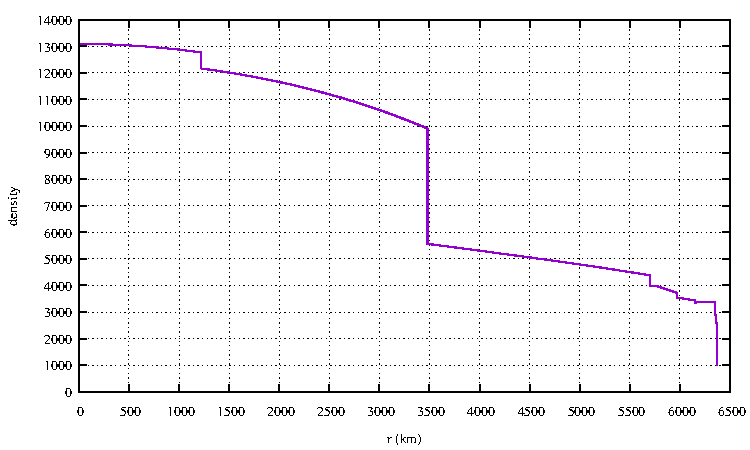
\includegraphics[width=8cm]{images/prem/rho.pdf}
\end{center}

\paragraph{Corresponding gravity field} Following Eq.~(\ref{eqn_g_rad_comp}), the radial component of the gravitational 
acceleration at a position $r$ outside of the Earth is given by:

\begin{equation}
g_r(r) 
= - \frac{1}{r^2} \int_0^r 4\pi {\cal G} \rho(r') r'^2 dr'
= - \frac{4 \pi {\cal G}}{r^2} \int_0^r \rho(r') r'^2 dr'
\end{equation}
 
This integral can be broken up into layer integrals and we can compute the contribution 
of each layer to the gravity value $g_r(r)$.
A layer is characterised by $r_{in}$ and $r_{out}$. Inside $r_{in}$ the gravity is zero. 
Between $r_{in}$ and $r_{out}$ the integral runs from $r_{in}$ to $r\leq r_{out}$. 
Anout outside the layer the integral runs from $r_{in}$ to $r_{out}$.

For simplicity the following integrals are computed for $x\in[0,1]$:

\begin{itemize}
\item inner core 

\begin{eqnarray}
inside \qquad g_{ic}(x)
&=& \frac{4 \pi {\cal G}}{x^2} \int_0^{x} (13.0885-8.8381 x'^2) x'^2 dx' \nn\\
&=& \frac{4 \pi {\cal G}}{x^2} (4.36283x^3-1.76762x^5) \nn\\
&=& 4 \pi {\cal G} (4.36283x-1.76762x^3) \\
outside \qquad g_{ic}(x)
&=&  \frac{4 \pi {\cal G}}{x^2} \int_0^{0.19172814314} (13.0885-8.8381 x'^2) x'^2 dx' \nn\\
&\simeq& 0.0302907  \frac{4 \pi {\cal G}}{x^2}
\end{eqnarray}



\item outer core 
\begin{eqnarray}
inside \qquad g_{oc}(x) 
&=& \frac{4 \pi {\cal G}}{x^2} \int_{0.19172814314}^{x} ( 12.5815-1.2638x'-3.6426x'^2-5.5281x'^3) x'^2 dx' \nn\\
&=& 4 \pi {\cal G} (-0.92135x^4 - 0.72852x^3 - 0.31595x^2+4.19383x-0.0288961/x^2) \\
outside \qquad g_{oc}(x)
&=&  \frac{4 \pi {\cal G} R^3}{x^2} 
\int_{0.19172814314}^{0.5462250824} (12.5815-1.2638x'-3.6426x'^2-5.5281x'^3)x'^2 dx'  \nn\\
&\simeq& 0.56663  \frac{4 \pi {\cal G}}{x^2}
\end{eqnarray}

\item lower mantle 
\begin{eqnarray}
inside \qquad g_{lm}(x)  &=& \frac{4 \pi {\cal G}}{x^2} \int_{}^{x} () x'^2 dx' \nn\\ 
outside \qquad g_{lm}(x) &=&  \frac{4 \pi {\cal G}}{x^2} \int_{}^{} () x'^2 dx' \nn\\  
\end{eqnarray}

\item transition zone 1 
\begin{eqnarray}
inside \qquad g_{lm}(x)  &=& \frac{4 \pi {\cal G}}{x^2} \int_{}^{x} () x'^2 dx' \nn\\ 
outside \qquad g_{lm}(x) &=&  \frac{4 \pi {\cal G}}{x^2} \int_{}^{} () x'^2 dx' \nn\\  
\end{eqnarray}

\item transition zone 2 
\begin{eqnarray}
inside \qquad g_{lm}(x)  &=& \frac{4 \pi {\cal G}}{x^2} \int_{}^{x} () x'^2 dx' \nn\\ 
outside \qquad g_{lm}(x) &=&  \frac{4 \pi {\cal G}}{x^2} \int_{}^{} () x'^2 dx' \nn\\  
\end{eqnarray}

\item transition zone 3 
\begin{eqnarray}
inside \qquad g_{lm}(x)  &=& \frac{4 \pi {\cal G}}{x^2} \int_{}^{x} () x'^2 dx' \nn\\ 
outside \qquad g_{lm}(x) &=&  \frac{4 \pi {\cal G}}{x^2} \int_{}^{} () x'^2 dx' \nn\\  
\end{eqnarray}


\end{itemize}


\begin{eqnarray}
g_{lm}(r) 
&=& \int_{3480/6371}^{5701/6371} (7.9565-6.4761x+5.5283x^2-3.0807x^3)x^2 dx 
\simeq 0.904793 \frac{4 \pi {\cal G} R^3}{r^2}\nn\\
g_{tz1}(r) 
&=& \int_{5701/6371}^{5771/6371} (5.3197-1.4836x)x^2 dx 
\simeq 0.0354823 \frac{4 \pi {\cal G} R^3}{r^2}\nn\\
g_{tz2}(r)
&=& \int_{5771/6371}^{5971/6371}   (11.2494-8.0298x)x^2 dx \simeq  0.1026 \frac{4 \pi {\cal G} R^3}{r^2}\nn\\
g_{tz3}(r)
&=& \int_{5971/6371}^{6151/6371}   (7.1089-3.8045x)x^2 dx  \simeq 0.0892215 \frac{4 \pi {\cal G} R^3}{r^2}\nn\\
g_{lvz} 
&=&  \int_{6151/6371}^{6291/6371} (2.6910+0.6924x) x^2 dx  \simeq  0.0705516 \frac{4 \pi {\cal G} R^3}{r^2}\nn\\
g_{lid}
&=& \int_{6291/6371}^{6346.6/6371} (2.6910+0.6924x)x^2 dx \simeq 0.0289968 \frac{4 \pi {\cal G} R^3}{r^2}\nn\\
g_{lc}
&=& \int_{6346.6/6371}^{6356/6371} 2.9 x^2 dx  \simeq 0.00425234 \frac{4 \pi {\cal G} R^3}{r^2}\nn\\
g_{uc}
&=& \int_{6356/6371}^{6368/6371} 2.6 x^2 dx  \simeq 0.00488337 \frac{4 \pi {\cal G} R^3}{r^2}\nn\\
g_{o}
&=& \int_{6368/6371}^{1} 1.020 x^2 dx  \simeq 0.000480075 \frac{4 \pi {\cal G} R^3}{r^2}
\end{eqnarray}


Finally 
\begin{eqnarray}
|g_r(r)| 
&=&  g_{ic}(r) + g_{oc}(r) + g_{lm}(r) + g_{tz1}(r) + g_{tz2}(r) + g_{tz3}(r) + 
g_{lvz}(r) + g_{lid}(r) + g_{lc}(r) + g_{uc}(r) + g_{o}(r) \nn\\
&=& 
\frac{4 \pi {\cal G} R^3}{r^2}
(
0.0302907 + 
0.56663 +
0.904793 +
0.0354823 +
0.1026 +
0.0892215+ \nn\\
&& 
0.0705516 +
0.0289968 +
0.00425234+
0.00488337+
0.000480075
  ) \nn\\
&\simeq& 
\frac{4 \pi {\cal G} R^3}{r^2} \nn
1.838181685
\end{eqnarray}

At the surface of the Earth, $r=R$ so we arrive at (after multiplying by 1000, see comment above): 
\[
\boxed{
g_{\tiny PREM}(R) \simeq 
4 \pi \cdot 6.67408\times 10^{-11}\cdot  6371\times 10^3 \cdot 1.838181685
\simeq 9.82194
}
\]

All these calculations should be rechecked, although obviously the obtained value makes much sense. 

